\documentclass[border=10pt]{standalone}
\usepackage{amsmath,amssymb}
\usepackage{tikz}
\usetikzlibrary{arrows.meta,calc,decorations.pathreplacing,decorations.pathmorphing,patterns,shapes.geometric,positioning,shadings,plotmarks}

\begin{document}
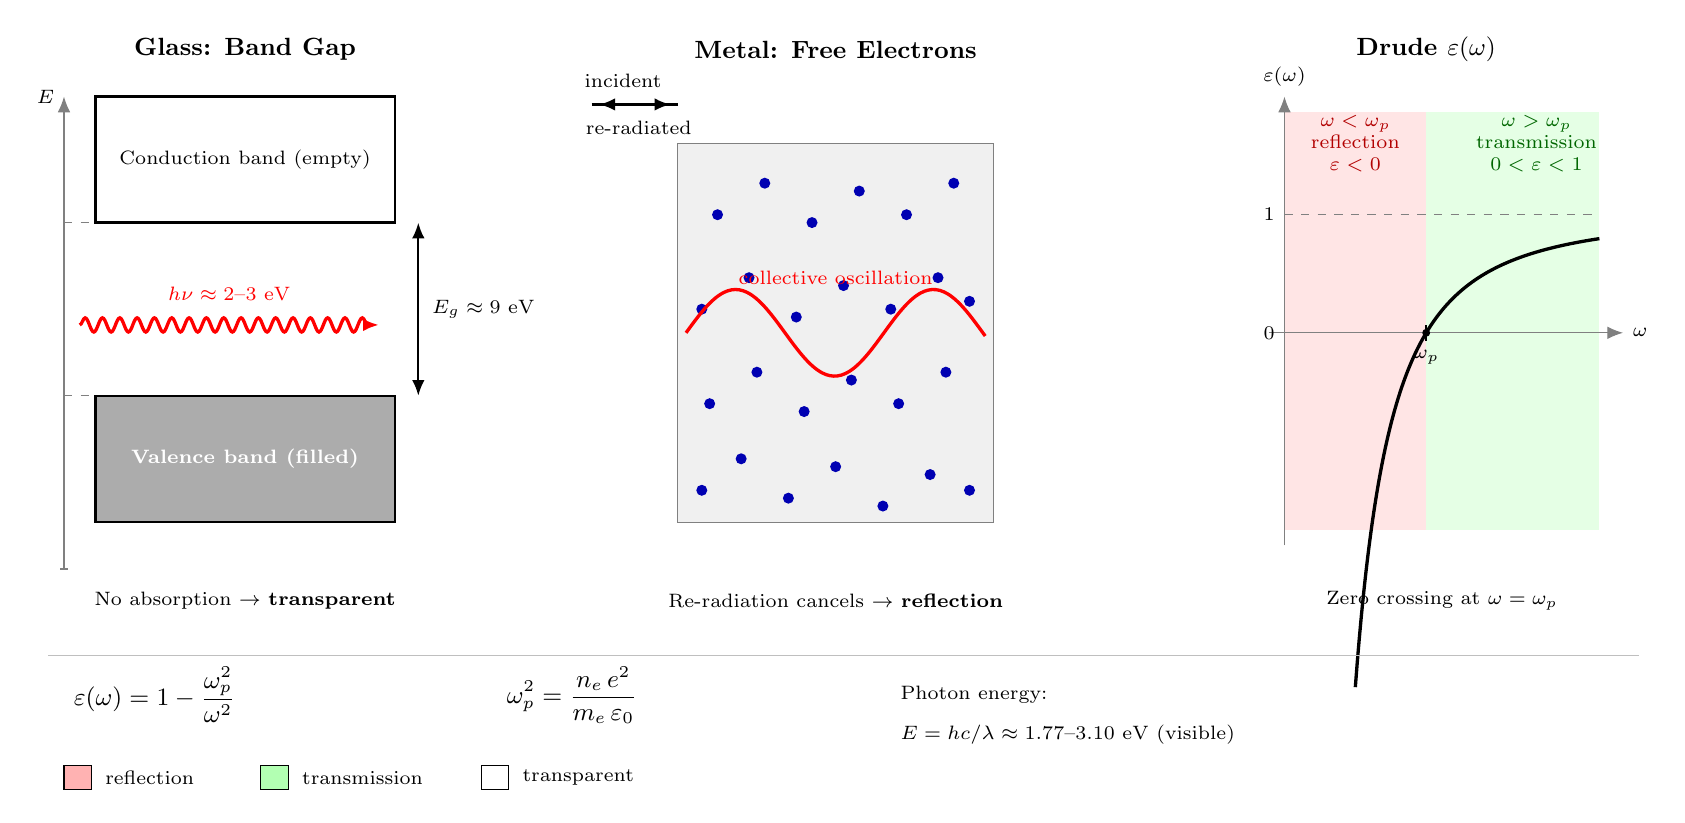
\begin{tikzpicture}[
  >={Latex[length=2mm,width=1.6mm]},
  font=\footnotesize
]

% ============================================================
% LEFT PANEL: Glass band gap
% ============================================================
\begin{scope}[shift={(0,0)}]
  \node[font=\small\bfseries] at (2.3,6.6) {Glass: Band Gap};

  % Axis (energy)
  \draw[->, gray] (0,0) -- (0,6) node[left,black,font=\scriptsize] {$E$};
  \draw[gray] (-0.05,0) -- (0.05,0);

  % Valence band (filled, dark gray)
  \fill[gray!65] (0.4,0.6) rectangle (4.2,2.2);
  \draw[black,thick] (0.4,0.6) rectangle (4.2,2.2);
  \node[white,font=\scriptsize\bfseries] at (2.3,1.4) {Valence band (filled)};

  % Conduction band (empty, hollow)
  \draw[black,thick] (0.4,4.4) rectangle (4.2,6.0);
  \node[black,font=\scriptsize] at (2.3,5.2) {Conduction band (empty)};

  % Band gap label
  \draw[<->, thick] (4.5,2.2) -- (4.5,4.4);
  \node[right,font=\scriptsize] at (4.55,3.3) {$E_g \approx 9~\mathrm{eV}$};

  % Dashed lines at band edges
  \draw[dashed,gray] (0,2.2) -- (0.4,2.2);
  \draw[dashed,gray] (0,4.4) -- (0.4,4.4);

  % Incoming photon arrow (short, below gap)
  \draw[->, red, very thick, decorate, decoration={snake,amplitude=0.9mm,segment length=2.2mm,post length=1.2mm}]
    (0.2,3.1) -- (4.0,3.1);
  \node[red,font=\scriptsize] at (2.1,3.5) {$h\nu \approx 2\text{--}3~\mathrm{eV}$};

  % Passes through label
  \node[font=\scriptsize, align=center] at (2.3,-0.4) {No absorption $\to$ \textbf{transparent}};
\end{scope}

% ============================================================
% MIDDLE PANEL: Metal electron sea
% ============================================================
\begin{scope}[shift={(7.5,0)}]
  \node[font=\small\bfseries] at (2.3,6.6) {Metal: Free Electrons};

  % Metal slab outline
  \draw[gray,thick] (0.3,0.6) rectangle (4.3,5.4);
  \fill[gray!12] (0.3,0.6) rectangle (4.3,5.4);

  % Electron dots (dark blue)
  \foreach \x/\y in {
    0.6/1.0, 1.1/1.4, 1.7/0.9, 2.3/1.3, 2.9/0.8, 3.5/1.2, 4.0/1.0,
    0.7/2.1, 1.3/2.5, 1.9/2.0, 2.5/2.4, 3.1/2.1, 3.7/2.5,
    0.6/3.3, 1.2/3.7, 1.8/3.2, 2.4/3.6, 3.0/3.3, 3.6/3.7, 4.0/3.4,
    0.8/4.5, 1.4/4.9, 2.0/4.4, 2.6/4.8, 3.2/4.5, 3.8/4.9
  } {
    \fill[blue!70!black] (\x,\y) circle (0.07);
  }

  % Sine wave (collective oscillation) across middle
  \draw[red, very thick, domain=0.4:4.2, samples=80, smooth]
    plot (\x, {3.0 + 0.55*sin(deg(2.5*(\x-0.4)))});

  % Incoming wave arrow (from left)
  \draw[->, black, thick] (-0.8,5.9) -- (0.2,5.9);
  \node[font=\scriptsize] at (-0.4,6.2) {incident};

  % Re-radiation arrow (backward, from metal)
  \draw[->, black, thick] (0.3,5.9) -- (-0.7,5.9);
  \node[font=\scriptsize] at (-0.2,5.6) {re-radiated};

  % Label for oscillation
  \node[red, font=\scriptsize] at (2.3,3.7) {collective oscillation};

  % Caption below
  \node[font=\scriptsize, align=center] at (2.3,-0.4) {Re-radiation cancels $\to$ \textbf{reflection}};
\end{scope}

% ============================================================
% RIGHT PANEL: Drude dielectric function curve
% ============================================================
\begin{scope}[shift={(15,0)}]
  \node[font=\small\bfseries] at (2.3,6.6) {Drude $\varepsilon(\omega)$};

  % Background shading regions
  \fill[red!10] (0.5,0.5) rectangle (2.3,5.8);
  \fill[green!10] (2.3,0.5) rectangle (4.5,5.8);

  % Axes
  \draw[->,gray] (0.3,3.0) -- (4.8,3.0) node[right,black,font=\scriptsize] {$\omega$};
  \draw[->,gray] (0.5,0.3) -- (0.5,6.0) node[above,black,font=\scriptsize] {$\varepsilon(\omega)$};

  % Zero line marker
  \node[left,font=\scriptsize] at (0.5,3.0) {$0$};
  \node[left,font=\scriptsize] at (0.5,4.5) {$1$};
  \draw[dashed,gray] (0.5,4.5) -- (4.5,4.5);

  % omega_p marker on x-axis
  \draw[thick] (2.3,2.9) -- (2.3,3.1);
  \node[below,font=\scriptsize] at (2.3,2.9) {$\omega_p$};

  % Curve: epsilon = 1 - wp^2 / w^2, with wp scaled so crossing at x=2.3
  % Let u = x - 0.5 (shift x-axis origin). Crossing at u = 1.8.
  % epsilon(u) = 1 - (1.8/u)^2. y = 3.0 + 1.5*epsilon
  % Plot from u = 0.9 to u = 4.0, i.e. x = 1.4 to 4.5
  \draw[black, very thick, domain=1.4:4.5, samples=120, smooth]
    plot (\x, {3.0 + 1.5*(1 - (1.8/(\x-0.5))*(1.8/(\x-0.5)))});

  % Asymptote to 1 visible
  % crossing point dot
  \fill[black] (2.3,3.0) circle (0.05);

  % Region labels
  \node[font=\scriptsize, red!70!black, align=center] at (1.4,5.4) {$\omega<\omega_p$\\reflection\\$\varepsilon<0$};
  \node[font=\scriptsize, green!40!black, align=center] at (3.7,5.4) {$\omega>\omega_p$\\transmission\\$0<\varepsilon<1$};

  % Caption below
  \node[font=\scriptsize, align=center] at (2.5,-0.4) {Zero crossing at $\omega=\omega_p$};
\end{scope}

% ============================================================
% BOTTOM: Key equations and legend
% ============================================================
\begin{scope}[shift={(0,-2.4)}]
  \draw[gray!50] (-0.2,1.3) -- (20,1.3);

  \node[anchor=west, font=\small] at (0,0.8)
    {$\displaystyle \varepsilon(\omega) = 1 - \frac{\omega_p^2}{\omega^2}$};

  \node[anchor=west, font=\small] at (5.5,0.8)
    {$\displaystyle \omega_p^2 = \frac{n_e\,e^2}{m_e\,\varepsilon_0}$};

  \node[anchor=west, font=\scriptsize] at (10.5,0.8) {Photon energy:};
  \node[anchor=west, font=\scriptsize] at (10.5,0.3) {$E = hc/\lambda \approx 1.77$--$3.10~\mathrm{eV}$ (visible)};

  % Legend boxes
  \fill[red!30] (0,-0.4) rectangle (0.35,-0.1);
  \draw[black] (0,-0.4) rectangle (0.35,-0.1);
  \node[anchor=west, font=\scriptsize] at (0.4,-0.25) {reflection};

  \fill[green!30] (2.5,-0.4) rectangle (2.85,-0.1);
  \draw[black] (2.5,-0.4) rectangle (2.85,-0.1);
  \node[anchor=west, font=\scriptsize] at (2.9,-0.25) {transmission};

  \fill[white] (5.3,-0.4) rectangle (5.65,-0.1);
  \draw[black] (5.3,-0.4) rectangle (5.65,-0.1);
  \node[anchor=west, font=\scriptsize] at (5.7,-0.25) {transparent};
\end{scope}

\end{tikzpicture}
\end{document}
